\documentclass[12pt]{article}
\usepackage{amsmath}
\usepackage{bm}
\usepackage{graphicx}
\usepackage{geometry}
\usepackage{indentfirst}
\usepackage{amsfonts}
\geometry{legalpaper, portrait, margin=0.5in}
\usepackage{color}   %May be necessary if you want to color links
\usepackage{hyperref}
\hypersetup{
    colorlinks=true, %set true if you want colored links
    linktoc=all,     %set to all if you want both sections and subsections linked
    linkcolor=black,  %choose some color if you want links to stand out
}
\usepackage[siunitx]{circuitikz}
\usetikzlibrary{patterns}
\usetikzlibrary{decorations.markings}
\graphicspath{ {./images/} }
\usepackage{amssymb}    
\newcommand{\sign}{\text{sign}}
\usepackage{enumitem}
\begin{document}
\newcommand*\dif{\mathop{}\!\mathrm{d}}

\setlist[enumerate]{noitemsep, topsep=0pt, leftmargin=2.5\parindent}
\setlist[itemize]{noitemsep, topsep=0pt, leftmargin=2.5\parindent}

\newenvironment{subitemize}
{ \begin{itemize}[leftmargin=\parindent] }
{ \end{itemize} }

\newenvironment{subenumerate}
{ \begin{enumerate}[leftmargin=\parindent] }
{ \end{enumerate} }

\newenvironment{nopagebr}
  {\par\nobreak\vfil\penalty0\vfilneg
   \vtop\bgroup}
  {\par\xdef\tpd{\the\prevdepth}\egroup
   \prevdepth=\tpd}

\tableofcontents

\addcontentsline{toc}{section}{Table of contents}
 
\pagebreak

\section{Modeling}

\subsection{Splines}

\subsubsection{Cubic Hermite Interpolation}

Each point is defined by its position $h_n$ and slope $h_{m + n}$, $m$ being the number of control points. To simplify calculations,
it is assumed that $t_0 = 0$ and $t_1 = 1$.

The goal is to convert from a monomial basis
\begin{align*}
    \phi_0(t) &= 1\\
    \phi_1(t) &= t\\
    \phi_2(t) &= t^2\\
    \phi_3(t) &= t^3
\end{align*}

to a hermite basis
\begin{align*}
    H_0(t) &= 2t^3 - 3t^2 + 1\\
    H_1(t) &= -2t^3 + 3t^2\\
    H_2(t) &= t^3 - 2t^2 + t\\
    H_3(t) &= t^3 - t^2
\end{align*}

so that instead of having to manipulate polynomial coefficients
\[ f(t) = a\phi_3(t) + b\phi_2(t) + c\phi_1(t) + d\phi_0(t) \]

an easier point slope method can be used:
\[ f(t) = h_0H_0(t) + h_1H_1(t) + h_2H_2(t) + h_3H_3(t) \]

\includegraphics[scale=.5]{images/cubic-hermite-interpolation.png}
\begin{align*}
    h_0 &= P(0) = d\\
    h_1 &= P(1) = a + b + c + d\\
    h_2 &= P'(0) = c\\
    h_3 &= P'(1) = 3a + 2b + c
\end{align*}

Unknowns in this equation are $a$, $b$, $c$, and $d$, so a matrix can be used
to solve the systems of equations:
\[
    \begin{pmatrix}
        0 & 0 & 0 & 1\\
        1 & 1 & 1 & 1\\
        0 & 0 & 1 & 0\\
        3 & 2 & 1 & 0
    \end{pmatrix}
    \begin{pmatrix}
        a\\
        b\\
        c\\
        d
    \end{pmatrix}
    =
    \begin{pmatrix}
        h_0\\
        h_1\\
        h_2\\
        h_3
    \end{pmatrix}
\]

$a$, $b$, $c$, and $d$ can be obtained from $h$ values by inverting the matrix:
\[
    \begin{pmatrix}
        0 & 0 & 0 & 1\\
        1 & 1 & 1 & 1\\
        0 & 0 & 1 & 0\\
        3 & 2 & 1 & 0
    \end{pmatrix}^{-1}
    \begin{pmatrix}
        h_0\\
        h_1\\
        h_2\\
        h_3
    \end{pmatrix}
    =
    \begin{pmatrix}
        a\\
        b\\
        c\\
        d
    \end{pmatrix}
\]

From these solved $h$ values, $P(t)$ can now be converted to a form that is
easier for a user to manipulate, in terms of $h$ values:
\begin{align*}
    P(t) =& \ at^3 + bt^2 + ct + d\\
    =& \ (2h_0 - 2h_1 + h_2 + h_3)t^3\\
        &+ (-3h_0 + 3h_1 - 2h_2 - h_3)t^2\\
        &+ h_2t + h_0\\
    =& \ h_0(2t^3 - 3t^2 + 1) + h_1(-2t^3 + 3t^2) +\\
       & \ h_2(t^3 - 2t^2 + t) + h_3(t^3 - t^2)
\end{align*}

Each equation in $P(t) = h_0(2t^3 - 3t^2 + 1) +
h_1(-2t^3 + 3t^2) + h_2(t^3 - 2t^2 + t) + h_3(t^3 - t^2)$ that is multiplied
by an $h$ value is called a cubic hermite.

\subsubsection{More than 1D}

A parametric curve described by $\vec \gamma(t) = (\gamma_0(t),
\gamma_1(t))$ can be converted into hermite basis like this:

\includegraphics[scale=.5]{images/parametric-hermite.png}

where cubic hermite interpolation can be done for both dimensions.

\subsubsection{Cubic blossom}

The cubic blossom of a function $\vec f(t)$ is $\vec F(t_1,t_2,t_3)$.

Cubic blossoms have three properties:
\begin{enumerate}
    \item Symmetric
        \begin{subitemize}
            \item $\vec F(t_1,t_2,t_3) = \vec F(t_1,t_3,t_2) = \vec F(t_3,t_1,t_2) \cdots$
        \end{subitemize}
    \item Affine
        \begin{subitemize}
            \item $\vec F(\alpha u + (1-\alpha)v,t_2,t_3) = \alpha \vec F(u,t_2,t_3) + 
                 (1-\alpha)\vec F(v,t_2,t_3)$
            \item If only one of $\vec F$'s arguments $t_c = \alpha u +
                (1-\alpha)v$ is changing between different points on $\vec F$,
                then any value $\vec F(t_c,t_2,t_3)$ in between $\vec F(u,t_2,t_3)$ and
                $\vec F(v,t_2,t_3)$ is scaled equivalently with $\alpha$ like
                $t_c$ is scaled between $u$ and $v$.
                
        \end{subitemize}
    \item Diagonal
        \begin{subitemize}
            \item $\vec f(t) = \vec F(t,t,t)$
        \end{subitemize}
\end{enumerate}

Blossoming examples
\begin{itemize}
    \item $\vec f(t) = t^3 \mapsto \vec F(t_1,t_2,t_3) = t_1t_2t_3$
    \item $\vec f(t) = t^2 \mapsto \vec F(t_1,t_2,t_3) = (t_1t_2 + 
            t_1t_3 + t_2t_3)/3$
    \item $\vec f(t) = t \mapsto \vec F(t_1,t_2,t_3) = (t_1 + t_2
            + t_3)/3$
    \item $\vec f(t) = 1 \mapsto \vec F(t_1,t_2,t_3) = 1$
    \item $\vec f(t) = 3t^3 - t + 1 = 3(t_1t_2t_3) - (t_1 + t_2
            + t_3)/3 + 1$
\end{itemize}

Cubic curves can be blossomed by blossoming each coordinate function
separately, which will give a function that maps 3 $t$ variables to
two dimensions $x$ and $y$: $\vec F(t_1,t_2,t_3): \mathbb R^3
\mapsto \mathbb R^2$. A cubic curve can be obtained from a blossom
by specifying four points $\vec F(0,0,0),\vec F(0,0,1),\vec F(0,1,1)
,\vec F(1,1,1)$ (which form a cubic control polygon) and subdividing
the surface given by the selected points (known as the De Castelijau's Algorithm).
Only these four points are required because of the symmetry property of a blossom.

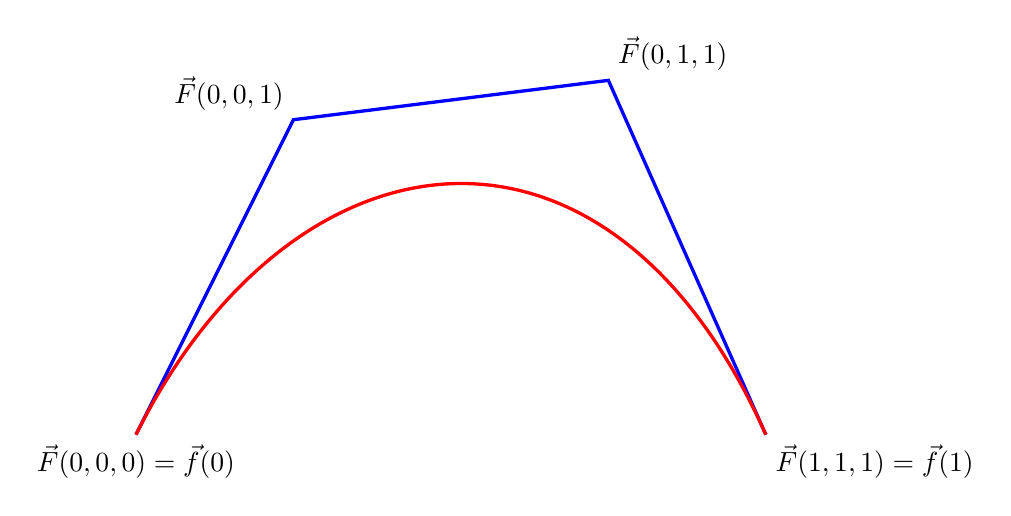
\begin{tikzpicture}
    \draw[color=blue, very thick] (0,0) -- (2,4)
        -- (6,4.5) -- (8,0);
    \draw[color=red, very thick] (0,0) .. controls (2,4) and (6, 4.5) .. (8,0);
    \node[anchor=north] at (0,0) {$\vec F(0,0,0) = \vec f(0)$};
    \node[anchor=south east] at (2,4) {$\vec F(0,0,1)$};
    \node[anchor=south west] at (6,4.5) {$\vec F(0,1,1)$};
    \node[anchor=north west] at (8,0) {$\vec F(1,1,1) = \vec f(1)$};
\end{tikzpicture}

Subdividing the polygon:

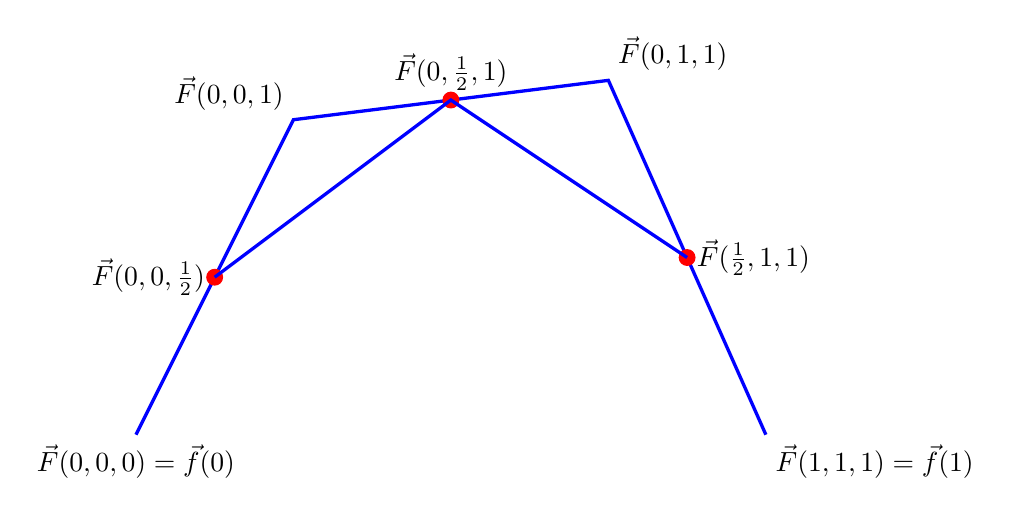
\begin{tikzpicture}
    \draw[color=blue, very thick] (0,0) -- (2,4)
        -- (6,4.5) -- (8,0);
    \node[anchor=north] at (0,0) {$\vec F(0,0,0) = \vec f(0)$};
    \node[anchor=south east] at (2,4) {$\vec F(0,0,1)$};
    \node[anchor=south west] at (6,4.5) {$\vec F(0,1,1)$};
    \node[anchor=north west] at (8,0) {$\vec F(1,1,1) = \vec f(1)$};

    \filldraw[color=red] (1,2) circle (0.1)
            node[color=black, anchor=east] {$\vec F(0,0,\frac 1 2)$};
    \filldraw[color=red] (4,4.25) circle (0.1)
            node[color=black, anchor=south] {$\vec F(0,\frac 1 2,1)$};
    \filldraw[color=red] (7,2.25) circle (0.1)
            node[color=black, anchor=west] {$\vec F(\frac 1 2, 1, 1)$};

    \draw[color=blue, very thick] (1,2) -- (4,4.25) -- (7,2.25);
\end{tikzpicture}

$\vec F$'s arguments at the subdivision points can be determined due to the affine
property of a blossom.

Further subdivision

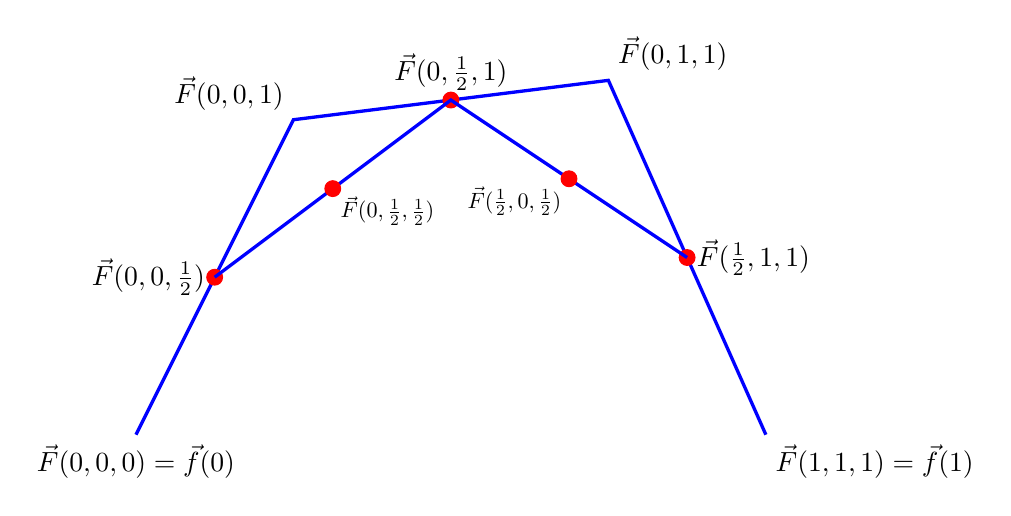
\begin{tikzpicture}
    \draw[color=blue, very thick] (0,0) -- (2,4)
        -- (6,4.5) -- (8,0);
    \node[anchor=north] at (0,0) {$\vec F(0,0,0) = \vec f(0)$};
    \node[anchor=south east] at (2,4) {$\vec F(0,0,1)$};
    \node[anchor=south west] at (6,4.5) {$\vec F(0,1,1)$};
    \node[anchor=north west] at (8,0) {$\vec F(1,1,1) = \vec f(1)$};

    \filldraw[color=red] (1,2) circle (0.1)
            node[color=black, anchor=east] {$\vec F(0,0,\frac 1 2)$};
    \filldraw[color=red] (4,4.25) circle (0.1)
            node[color=black, anchor=south] {$\vec F(0,\frac 1 2,1)$};
    \filldraw[color=red] (7,2.25) circle (0.1)
            node[color=black, anchor=west] {$\vec F(\frac 1 2, 1, 1)$};

    \draw[color=blue, very thick] (1,2) -- (4,4.25) -- (7,2.25);

    \filldraw[color=red] (2.5,3.125) circle (0.1)
            node[color=black, anchor=north west, scale=.8] {$\vec F(0,\frac 1 2,\frac 1 2)$};
    \filldraw[color=red] (5.5,3.25) circle (0.1)
            node[color=black, anchor=north east, scale=.8] {$\vec F(\frac 1 2, 0, \frac 1 2)$};
\end{tikzpicture}

One more subdivision (most recent two subdivision point values omitted
because there's no room left)

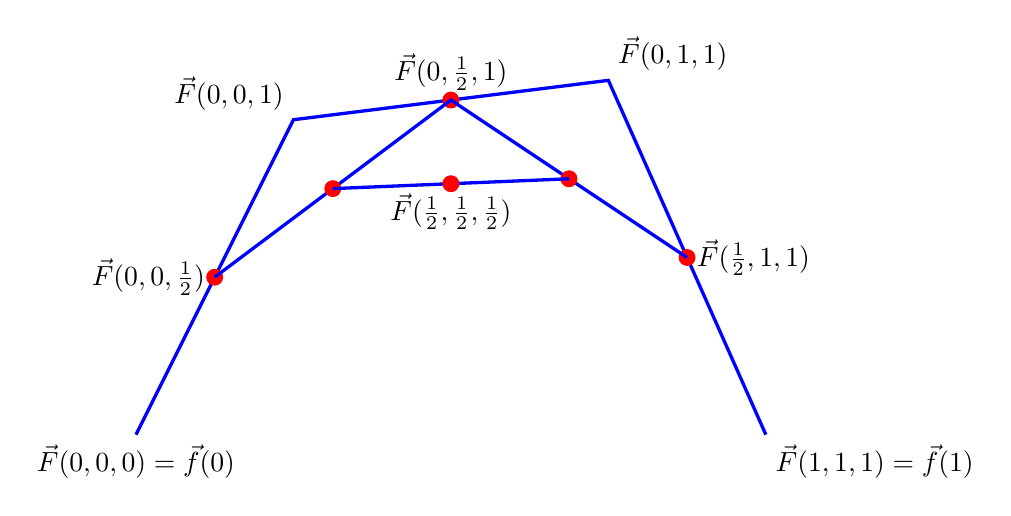
\begin{tikzpicture}
    \draw[color=blue, very thick] (0,0) -- (2,4)
        -- (6,4.5) -- (8,0);
    \node[anchor=north] at (0,0) {$\vec F(0,0,0) = \vec f(0)$};
    \node[anchor=south east] at (2,4) {$\vec F(0,0,1)$};
    \node[anchor=south west] at (6,4.5) {$\vec F(0,1,1)$};
    \node[anchor=north west] at (8,0) {$\vec F(1,1,1) = \vec f(1)$};

    \filldraw[color=red] (1,2) circle (0.1)
            node[color=black, anchor=east] {$\vec F(0,0,\frac 1 2)$};
    \filldraw[color=red] (4,4.25) circle (0.1)
            node[color=black, anchor=south] {$\vec F(0,\frac 1 2,1)$};
    \filldraw[color=red] (7,2.25) circle (0.1)
            node[color=black, anchor=west] {$\vec F(\frac 1 2, 1, 1)$};

    \draw[color=blue, very thick] (1,2) -- (4,4.25) -- (7,2.25);
    \filldraw[color=red] (2.5,3.125) circle (0.1);
    \filldraw[color=red] (5.5,3.25) circle (0.1);
    \draw[color=blue, very thick] (2.5,3.125) -- (5.5,3.25);
    \filldraw[color=red] (4,3.1875) circle (0.1)
            node[color=black, anchor=north] {$\vec F(\frac 1 2, \frac 1 2
            , \frac 1 2)$};
\end{tikzpicture}

The final subdivision point can be shown to equal $\vec f(\frac 1 2)$
because of the diagonal property of blossoms, meaning the $\vec f$ curve
will intersect this third subdivision point:

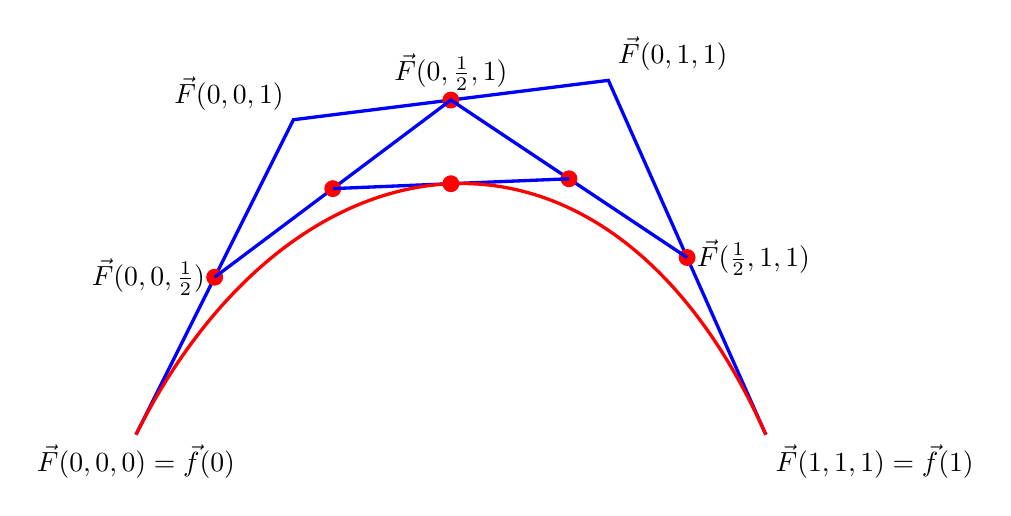
\begin{tikzpicture}
    \draw[color=blue, very thick] (0,0) -- (2,4)
        -- (6,4.5) -- (8,0);
    \node[anchor=north] at (0,0) {$\vec F(0,0,0) = \vec f(0)$};
    \node[anchor=south east] at (2,4) {$\vec F(0,0,1)$};
    \node[anchor=south west] at (6,4.5) {$\vec F(0,1,1)$};
    \node[anchor=north west] at (8,0) {$\vec F(1,1,1) = \vec f(1)$};

    \filldraw[color=red] (1,2) circle (0.1)
            node[color=black, anchor=east] {$\vec F(0,0,\frac 1 2)$};
    \filldraw[color=red] (4,4.25) circle (0.1)
            node[color=black, anchor=south] {$\vec F(0,\frac 1 2,1)$};
    \filldraw[color=red] (7,2.25) circle (0.1)
            node[color=black, anchor=west] {$\vec F(\frac 1 2, 1, 1)$};

    \draw[color=blue, very thick] (1,2) -- (4,4.25) -- (7,2.25);
    \filldraw[color=red] (2.5,3.125) circle (0.1);
    \filldraw[color=red] (5.5,3.25) circle (0.1);
    \draw[color=blue, very thick] (2.5,3.125) -- (5.5,3.25);

    \filldraw[color=red] (4,3.1875) circle (0.1);
    \draw[color=red, very thick] (0,0) .. controls (2,4) and (6, 4.5) .. (8,0);
\end{tikzpicture}

Other values of $\vec f$ can be found with subdividing the cubic control
polygon on different values. For example, to find $\vec f(\frac 1 4)$,
each edge would be divided $\frac 1 4$ of the way along it.

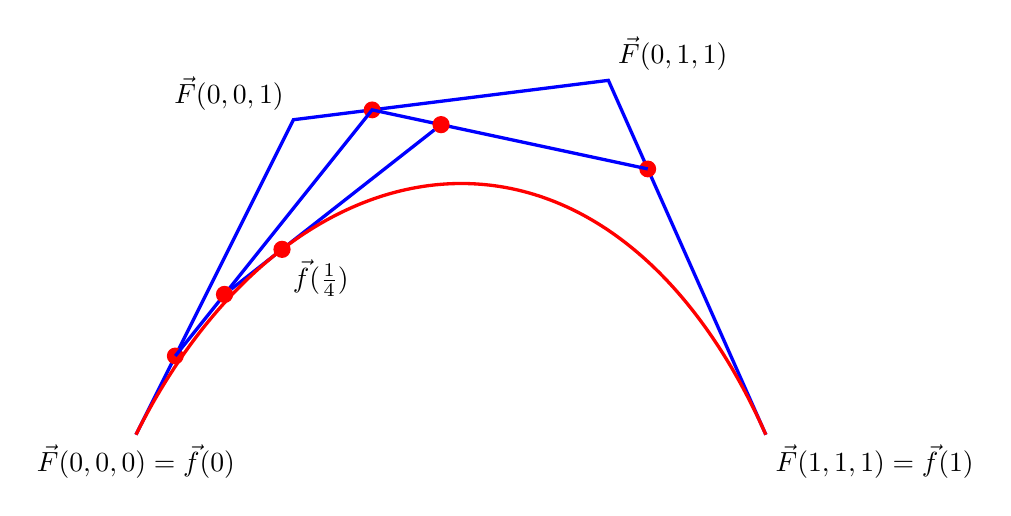
\begin{tikzpicture}
    \draw[color=blue, very thick] (0,0) -- (2,4)
        -- (6,4.5) -- (8,0);
    \node[anchor=north] at (0,0) {$\vec F(0,0,0) = \vec f(0)$};
    \node[anchor=south east] at (2,4) {$\vec F(0,0,1)$};
    \node[anchor=south west] at (6,4.5) {$\vec F(0,1,1)$};
    \node[anchor=north west] at (8,0) {$\vec F(1,1,1) = \vec f(1)$};

    \filldraw[color=red] (.5,1) circle (0.1);
    \filldraw[color=red] (3,4.125) circle (0.1);
    \filldraw[color=red] (6.5,3.375) circle (0.1);

    \draw[color=blue, very thick] (.5,1) -- (3,4.125)
        node[pos=.25,draw=red,fill=red,shape=circle,
        minimum size=5pt,inner sep=0pt] (A) {} -- (6.5,3.375)
        node[pos=.25,draw=red,fill=red,shape=circle,
        minimum size=5pt,inner sep=0pt] (B) {};
    \draw[color=blue, very thick] (A) -- (B)
        node[pos=.25, draw=red,fill=red,shape=circle,
        minimum size=5pt,inner sep=0pt] {} node[pos=.25,anchor=north west,
        color=black] {$\vec f(\frac 1 4)$};

    \draw[color=red, very thick] (0,0) .. controls (2,4) and (6, 4.5) .. (8,0);
\end{tikzpicture}

\subsubsection{Bernstein polynomials}

Another basis that can represent cubic curves. Bernstein basis is
canonical for Bezier.

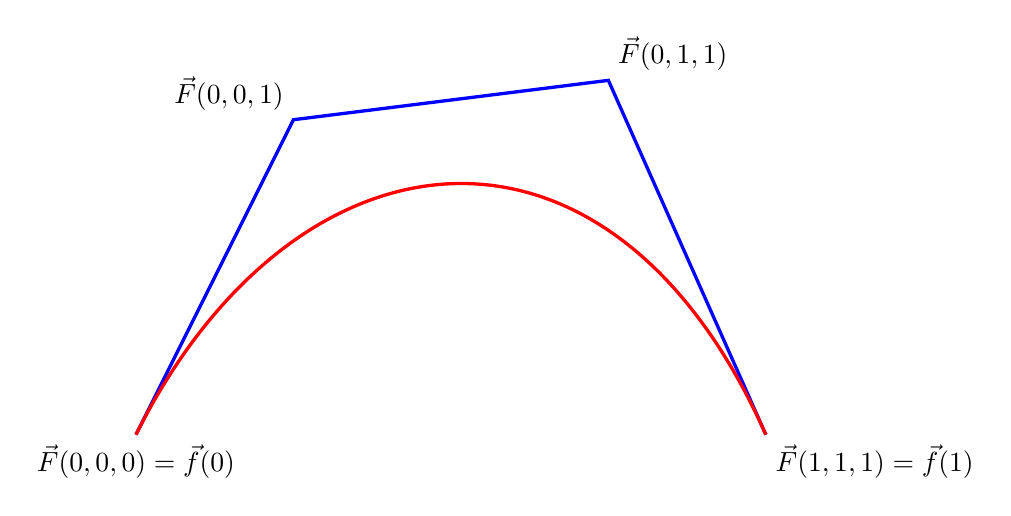
\begin{tikzpicture}
    \draw[color=blue, very thick] (0,0) -- (2,4)
        -- (6,4.5) -- (8,0);
    \draw[color=red, very thick] (0,0) .. controls (2,4) and (6, 4.5) .. (8,0);
    \node[anchor=north] at (0,0) {$\vec F(0,0,0) = \vec f(0)$};
    \node[anchor=south east] at (2,4) {$\vec F(0,0,1)$};
    \node[anchor=south west] at (6,4.5) {$\vec F(0,1,1)$};
    \node[anchor=north west] at (8,0) {$\vec F(1,1,1) = \vec f(1)$};
\end{tikzpicture}

The red curve above can be represented as $\vec f(t) = \vec F(0,0,0)
B_0(t) + \vec F(0,0,1)B_1(t) + \vec F(0,1,1)B_2(t) + F(1,1,1)B_3(t)$, 
knowing
\begin{align*}
    B_0(t) &= (1-t)^3 = 1-3t+3t^2-t^3\\
    B_1(t) &= 3t(1-t)^2 = 3t-6t^2+3t^3\\
    B_2(t) &= 3t^2(1-t) = 3t^2-3t^3\\
    B_3(t) &= t^3
\end{align*}

Changing basis from monomial to Bernstein:
\[
    \begin{pmatrix}
        1 & -3 & 3 & -1\\
        0 & 3 & -6 & 3\\
        0 & 0 & 3 & -3\\
        0 & 0 & 0 & 1
    \end{pmatrix}
    \begin{pmatrix}
        1\\
        t\\
        t^2\\
        t^3
    \end{pmatrix}
    =
    \begin{pmatrix}
        B_0(t)\\
        B_1(t)\\
        B_2(t)\\
        B_3(t)
    \end{pmatrix}
\]

And to change from Bernstein to monomial, the inverse of the matrix
can be used.

\subsubsection{General spline formulation}

$\vec \gamma(t) =$ Geometry $\cdot$ Spline basis $\cdot$ Monomial basis
\begin{itemize}
    \item Geometry contains control point coordinates
    \item Spline basis defines the type of spline (Hermite, Bernstein, etc)
    \item Monomial basis is a column vector $(1,t,t^2,\cdots,t^n)$
\end{itemize}

Example of a spline represented in the Bernstein basis:
\[
    P(t) =
    \begin{pmatrix}
        x(t)\\
        y(t)
    \end{pmatrix}
    =
    \begin{pmatrix}
        x_1 & x_2 & x_3 & x_4\\
        y_1 & y_2 & y_3 & y_4
    \end{pmatrix}
    \begin{pmatrix}
        1 & -3 & 3 & -1\\
        0 & 3 & -6 & 3\\
        0 & 0 & 3 & -3\\
        0 & 0 & 0 & 1
    \end{pmatrix}
    \begin{pmatrix}
        1\\
        t\\
        t^2\\
        t^3
    \end{pmatrix}
\]

\subsubsection{Orders of continuity}

$C^0$ = continuous (seam can be sharp)

$G^1$ = geometric continuity (Tangent vectors align at the seam)

$C^1$ = parametric continuity (Same velocity at the seam)

$C^2$ = curvature continuity (Tangents and tangent derivatives are the same)

\subsubsection{Cubic B-splines}

$\ge$ 4 control points

Chain together splines in fours, popping the back control point off and
pushing the next control point on

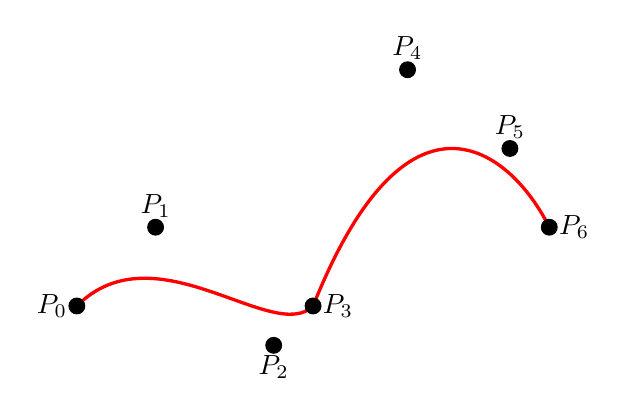
\begin{tikzpicture}
    \draw[color=red,very thick] (0,0) .. controls (1, 1) and (2.5, -.5)
        .. (3, 0) .. controls (4.2,3) and (5.5,2) .. (6,1);
    \filldraw (0,0) circle (.1) node[anchor=east] {$P_0$};
    \filldraw (1,1) circle (.1) node[anchor=south] {$P_1$};
    \filldraw (2.5,-.5) circle (.1) node[anchor=north] {$P_2$};
    \filldraw (3,0) circle (.1) node[anchor=west] {$P_3$};
    \filldraw (4.2,3) circle (.1) node[anchor=south] {$P_4$};
    \filldraw (5.5,2) circle (.1) node[anchor=south] {$P_5$};
    \filldraw (6,1) circle (.1) node[anchor=west] {$P_6$};
\end{tikzpicture}

The full curve is composed of many smaller splines, in which the
$n$th spline is formed by points $P_{n..n+3}$. The benefit of this
method is that it guarantees $C^1$ continuity since every spline shares
three control points with the one that comes before and after it.

The end points won't connect with this method, but repeating endpoints
will fix it.

The basis functions as well as the basis conversion matrix
for cubic b-spline are listed here:
\begin{align*}
    B_1(t) &= \frac 1 6 (1-t)^3\\
    B_2(t) &= \frac 1 6 (3t^3-6t^2+4)\\
    B_3(t) &= \frac 1 6 (-3t^3+3t^2+3t+1)\\
    B_4(t) &= \frac 1 6 t^3
\end{align*}
\[
    B_{B-spline} =
    \frac 1 6
    \begin{pmatrix}
        1 & -3 & 3 & -1\\
        4 & 0 & -6 & 3\\
        1 & 3 & 3 & -3\\
        0 & 0 & 0 & 1
    \end{pmatrix}
\]

\subsubsection{Bezier vs B-spline}

\includegraphics[scale=.5]{images/bezier-vs-bspline.png}

Bezier is derived from Bernstein polynomials, while B-spline uses a
different set of basis functions. Additionally, Bezier will try
to intersect with control points and only guarantees $C^0$ continuity,
while B-spline does not and guarantees $C^1$ continuity.

Converting between bezier and b-spline, given $G$ = geometry,
$B_0$ = current basis matrix, $T(t)$ = monomial basis, and $B_1$ =
the basis matrix to convert to:
\begin{align*}
    \vec \gamma(t) &= G \cdot B_0 \cdot T(t)\\
    &= G \cdot B_0 \cdot B_1^{-1} \cdot B_1 \cdot T(t)\\
    &= (G \cdot B_0 \cdot B_1^{-1}) \cdot B_1 \cdot T(t)
\end{align*}

The new geometry matrix is then represented as $G \cdot B \cdot
B_1^{-1}$, which shows that to convert between bezier and b-spline,
a different set of data is required for the same curve.

\subsection{2D Surfaces}

\subsubsection{Bicubic Bezier surfaces}
\includegraphics[scale=2]{images/surface-example.png}

Given $u$ changes vertically and $v$ changes horizontally,
\begin{align*}
    P(u,v) =& \ (1-u)^3 P_1(v)\\
    &+ 3u(1-u)^2 P_2(v)\\
    &+ 3u^2(1-u) P_3(v)\\
    &+ u^3 P_4(v)
\end{align*}

For any constant $u$ for $0 \le u \le 1$ there is a bezier curve
as a function of $v$ for $0 \le v \le 1$ at that $u$, and vice
versa.

\includegraphics[scale=2]{images/bicubic-bezier-surface.png}
\begin{align*}
    P(u,v) &= \sum_{i=1}^4 B_i(u) P_i(v)\\
    P_i(v) &= \sum_{j=1}^4 B_j(v) P_{i,j}
\end{align*}

Which can be compactly expressed as:
\begin{align*}
    P(u,v) &= \sum_{i=1}^4 B_i(u) \left[ \sum_{j=1}^4 P_{i,j} B_j(v) \right]\\
           &= \sum_{i=1}^4 \sum_{j=1}^4 P_{i,j} B_{i,j}(u,v)
\end{align*}

where $B_{i,j}(u,v) = B_i(u)B_j(v)$.

\subsubsection{Tangents and Normals for patches}

The partial derivatives $\partial P/\partial u$ and
$\partial P/\partial v$ are tangent vectors.

Normal vector is equal to the cross product of the tangent vectors:
\[ \vec N = \frac{\partial P}{\partial u} \times \frac{\partial P}
{\partial v} \]

$\vec N$ is typically not unit, so it needs to be normalized

\subsubsection{Matrix notation for patches}
\[
    P(u,v) =
    \begin{pmatrix}
        B_1(u) & \cdots & B_4(u)
    \end{pmatrix}
    \begin{pmatrix}
        P_{1,1} & \cdots & P_{1,4}\\
        \vdots & \ddots & \vdots\\
        P_{4,1} & \cdots & P_{4,4}
    \end{pmatrix}
    \begin{pmatrix}
        B_1(v)\\
        \vdots\\
        B_4(v)
    \end{pmatrix}
\]

\subsubsection{Implicit surfaces}

$f(x,y,z) = 0$ is on the surface

$f(x,y,z) < 0$ is inside the surface

$f(x,y,z) > 0$ is outside the surface

\subsection{Hierarchical modeling}

\subsubsection{Forward kinematics}

Specifies base position and joint angles. To compute the final position
and orientation of a joint in world coordinates, the motion of all its
ancestor joints must be computed as well.

Given values for joint dof (degree of freedom) $\vec \theta = [\theta_1,\theta_2,
\cdots,\theta_n]^T$, compute the end effector in world space $\vec{\bm e} =
[\bm e_1,\bm e_2,\cdots,\bm e_m]^T$.

$\vec{\bm e} = F(\bm \theta)$

\includegraphics[scale=2]{images/arm.png}

In the diagram above, $P$ in world coordinates can be calculated with
$P_{world} = M_{01}M_{12}M_{23}P_{local}$, or $T(0,6)R(-45)T(5,0)R(50)
T(4,0)R(30)P_{local}P_{local}$, $T$ being a transformation matrix and $R$
being a rotation matrix.

\subsubsection{Inverse kinematics}

Forward kinematics has some issues such as determining what orientation
the arm should be in to interact with other objects, which is what
inverse kinematics aims to solve.

In forward kinematics, $(\bm e_1,\bm e_2) = F(\theta_1,\theta_2,\theta_3)$;
however, in inverse kinematics, $(\theta_1,\theta_2,\theta_3) = G(\bm e_1,
\bm e_2)$.

Inverse kinematics is difficult because sometimes there is no solution / multiple
solutions to a problem. Typically it can't be analytically solved and requires numerical methods.
\begin{itemize}
    \item Jacobian iterative method
    \item Optimization based methods
\end{itemize}

Given position of a point in local coordinates $\bm v_s$ and desired
position in world coordinates $\bm v_w$, find skeleton parameters
$\bm p$.
\[ \bm v_w = S(\bm p)\bm v_s = S(x_h,y_h,z_h,\theta_h,\phi_h,\sigma_h,
\theta_t,\phi_t,\sigma_t,\theta_c,\theta_f,\phi_f) \bm v_s \]

\subsubsection{Jacobian}

$\bm e = F(\bm \theta)$ where $\bm e$ is known and $\bm \theta$
is to be solved for.

The Jacobian is the matrix of partial derivatives
of $\bm F$: $J = \dif F/\dif \bm \theta$

For $\bm F = [\bm F_1,\bm F_2,\cdots,\bm F_m]^T$ and $\bm \theta
= [\theta_1,\theta_2,\cdots,\theta_n]^T$:
\[
    J =
    \begin{bmatrix}
        \frac{\partial \bm F_1}{\partial \theta_1} & \cdots & \frac{\partial F_1}{\partial \theta_n}\\
        \vdots & \ddots & \vdots\\
        \frac{\partial F_m}{\partial \theta_1} & \cdots & \frac{\partial F_m}{\partial \theta_n}
    \end{bmatrix}
\]

\subsection{Skinning}

\subsubsection{SSD}

Skin is made up of vertices, some of which are attached
to a single bone, while others are attached to multiple.

Example

\includegraphics[scale=.4]{images/skinning-vertices.png}

\subsubsection{Vertex weights}

Weight $w_{ij}$ is assigned for each vertex $\bm p_i$ for each
bone $\bm b_j$. ("How much will vertex $i$ move with bone $j$?")

$w_{ij} = 1$ means $\bm p_i$ is rigidly attached to bone $\bm b_j$.
Weights should not be negative, and the sum of weights across
all bones for each vertex should equal 1.

The number of bones that can influence a single vertex is typically
limited to $N = 4$ bones/vertex.

\subsubsection{Linear blend skinning}

First transform each vertex $\bm p_i$ with each bone as if it were
tied to it rigidly, and then blend the results using weights.

Given $\bm p'_{ij}$ is vertex $i$ transformed by bone $j$, $T_j$ is
the current transformation of bone $j$, and $\bm p'_i$ is the new
position of vertex $i$:
\begin{align*}
    \bm p'_{ij} &= T_j \bm p_i\\
    \bm p'_i &= \sum_j w_{ij} \bm p'_{ij}
\end{align*}

Example

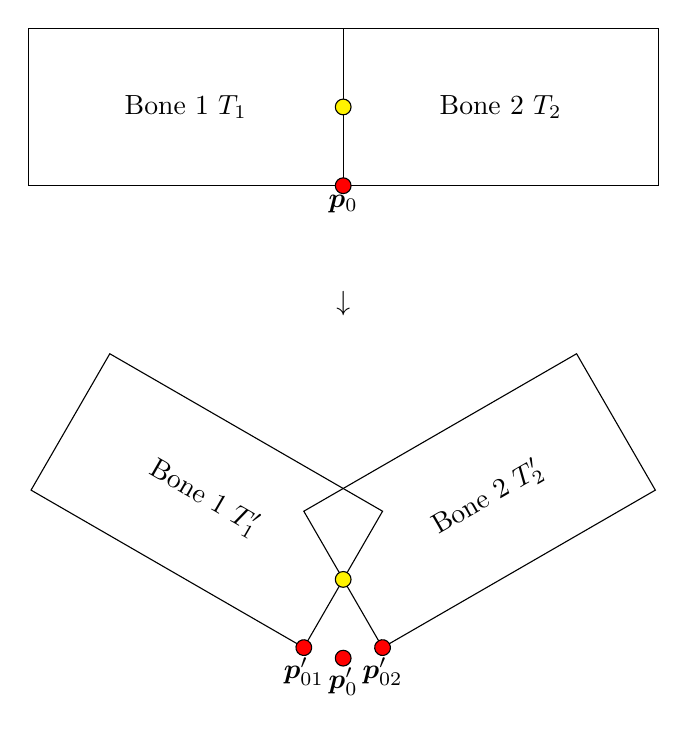
\begin{tikzpicture}
    \draw (0,0) rectangle (4,2);
    \draw (4,0) rectangle (8,2);
    \node at (2,1) {Bone 1 $T_1$};
    \node at (6,1) {Bone 2 $T_2$};
    \filldraw[draw=black,fill=red] (4,0) circle (.1) node[anchor=north]
    {$\bm p_0$};
    \filldraw[draw=black,fill=yellow] (4,1) circle (.1);

    \node at (4,-1.5) {$\downarrow$};

    \draw[rotate around={-30:(4,-5)}] (4,-6) rectangle (0,-4);
    \draw[rotate around={30:(4,-5)}] (4,-6) rectangle (8,-4);
    \node[rotate around={-30:(4,-5)}] at (-0.8,-5.3) {Bone 1 $T'_1$};
    \node[rotate around={30:(4,-5)}] at (7.8,-1.3) {Bone 2 $T'_2$};
    \filldraw[draw=black,fill=yellow] (4,-5) circle (.1);

    \filldraw[draw=black,fill=red,rotate around={-30:(4,-5)}] (4,-6)
        circle (.1) node[anchor=north] (A) {$\bm p'_{01}$};
    \filldraw[draw=black,fill=red,rotate around={30:(4,-5)}] (4,-6)
        circle (.1) node[anchor=north] (B) {$\bm p'_{02}$};
    \filldraw[draw=black,fill=red] (4,-6) circle(.1) node[anchor=north]
        (C) {$\bm p'_0$};
\end{tikzpicture}

Vertex $\bm p_0$ has weights $w_{01} = 0.5$ and $w_{02} = 0.5$. Points
$\bm p'_{01}$ and $\bm p'_{02}$ are generated by transforming point
$\bm p_0$ using $T'_1$ and $T'_2$. $\bm p'_0$ can be determined using
$\bm p'_0 = w_{01}\bm p'_{01} + w_{02}\bm p'_{02} = 0.5\bm p'_{01} + 0.5
\bm p'_{02}$.

\section{Raytracing}

\subsection{Geometry representation}

A ray is represented as $\bm p(t) = \bm R_o + \bm R_d t$, $\bm R_o$
being the ray origin and $\bm R_d$ being the ray direction. All
solutions for $t$ under section 2.1 refer
to the $t$ parameter for $\bm p(t)$.

Implicit equations $H(\bm P)$ are boolean functions.
For example, given the implicit equation $H(\bm P) = \bm a \cdot \bm P = 0$,
$H(\bm P)$ returns $\bm a \cdot \bm P \le 0$.

For the computation of intersections with any object, the object should be
assumed to be at the origin, with the ray being transformed by the inverse
of the object transformation matrix, as well as the ray direction.
For point transformation, use $w = 1$, and direction transformation
$w = 0$ because direction transformation doesn't include translation.

If ray direction is normalized, $t_{ws} \ne t_{os}$.
and must be rescaled after the intersection. If ray direction is not normalized,
$t_{ws} = t_{os}$, which is why it's preferred to not normalize
transformed ray direction.

\includegraphics[scale=.5]{images/raytrace-world-to-object.png}

To transform object normals properly, use $\bm n_{ws} = (M^{-1})^T \bm
n_{os}$.

\subsubsection{Sphere}

Implicit equation: $H(\bm P) = \bm P \cdot \bm P - r^2 = 0$

Intersection detection ($r$ is sphere radius)
\begin{gather*}
    a = \bm R_d \cdot \bm R_d\\
    b = 2(-\bm R_o \cdot \bm R_d)\\
    c = \bm R_o \cdot \bm R_o - r^2\\
    d = b^2 - 4ac\\
    t = \frac{-b \pm \sqrt{d}}{2a}
\end{gather*}

If $d < 0$, there is no intersection. If both solutions for $t$
are negative, there is no intersection.
If only one solution for $t$ is positive, that is where the
intersection occurs. If both solutions for $t$ are positive,
the intersection occurs at the closest $t$.

\subsubsection{Infinite plane}

Implicit equation: $H(\bm P) = \bm n \cdot \bm P + D = 0$, with $\bm n$
= plane normal, $D = -(\bm n \cdot \bm P_0)$, $\bm P_0$ = some point on
the plane.

If there is an intersection, $\bm n \cdot \bm P + D$ gives the distance from
$\bm P$ to $\bm P_0$.

\subsubsection{Triangle}

Any point $\bm P$ on a triangle $(\bm a,\bm b,\bm c)$ can be represented as $\bm P(
\alpha,\beta,\gamma) = \alpha \bm a + \beta \bm b + \gamma \bm
c$, with $\alpha + \beta + \gamma = 1$.

If $\alpha$, $\beta$, $\gamma$ $\ge 0$ then the barycentric coordinates are inside
the triangle.

\textbf{Computation of $\alpha$, $\beta$, $\gamma$ - geometric approach} ($A$ = area
of entire triangle, $A_x$ = area of subsection of triangle opposite to
triangle vertex $\bm x$, $\bm P$ = random point on triangle)

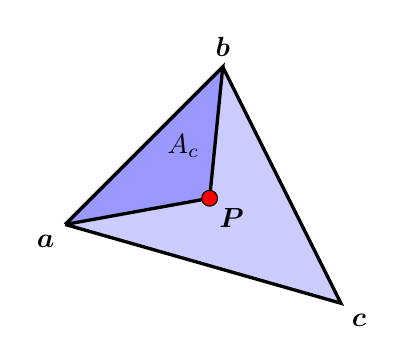
\begin{tikzpicture}
    \filldraw[fill=white!80!blue,very thick] (0,0) node[anchor=north east]
        {$\bm a$} -- (2,2) node[anchor=south] {$\bm b$} -- (3.5,-1)
        node[anchor=north west] {$\bm c$} -- (0,0);
    \filldraw[fill=white!60!blue,very thick] (0,0) -- (2,2) -- (1.833,0.333)
        -- (0,0);
    \filldraw[fill=red,draw=black] (1.833,0.333) circle (.1) node[anchor=north west]
        {$\bm P$};
    \node at (1.5,1) {$A_c$};
\end{tikzpicture}

\begin{align*}
    \alpha &= \frac{A_a}{A}\\
    \beta &= \frac{A_b}{A}\\
    \gamma &= \frac{A_c}{A}
\end{align*}

\textbf{Computation of $\alpha$, $\beta$, $\gamma$ - algebraic approach}

Since $\alpha$, $\beta$, and $\gamma$ sum to 1, $\alpha = 1 - \beta - \gamma$,
allowing for $\bm P(\alpha,\beta,\gamma)$ to be written as $\bm P(\beta,
\gamma) = (1-\beta-\gamma)\bm a + \beta \bm b + \gamma \bm c$, or
$\bm P(\beta,\gamma) = \bm a + \beta (\bm b - \bm a) + \gamma (\bm c
- \bm a)$. To simplify, $\bm P(\beta,\gamma)$ can also be written as
$\bm a + \beta \vec e_1 + \gamma \vec e_2$, where $\vec e$ is an edge vector.
\begin{gather*}
    \bm P = \bm a + \beta \vec e_1 + \gamma \vec e_2\\
    \vec e_1 \cdot (\bm P - \bm a) = \vec e_1 \cdot (\beta \vec e_1 + \gamma \vec e_2)\\
    \vec e_2 \cdot (\bm P - \bm a) = \vec e_2 \cdot (\beta \vec e_1 + \gamma \vec e_2)\\
    \begin{pmatrix}
        \vec e_1 \cdot (\bm P - \bm a)\\
        \vec e_2 \cdot (\bm P - \bm a)
    \end{pmatrix}
    =
    \begin{pmatrix}
        \vec e_1 \cdot \vec e_1 & \vec e_1 \cdot \vec e_2\\
        \vec e_2 \cdot \vec e_1 & \vec e_2 \cdot \vec e_2
    \end{pmatrix}
    \begin{pmatrix}
        \beta\\
        \gamma
    \end{pmatrix}
\end{gather*}

Intersection with barycentric triangle - set ray equal to barycentric equation
\begin{gather*}
    \bm P(t) = \bm P(\beta,\gamma)\\
    \bm R_0 + t \bm R_d = \bm a + \beta (\bm b - \bm a) + \gamma
    (\bm c - \bm a)
\end{gather*}

Intersection if $\beta + \gamma \le 1$, $\beta \ge 0$, $\gamma \ge 0$

Separate equation into x, y, z components and turn it into matrix
form:
\[
    \begin{pmatrix}
        \bm a_x - \bm R_{ox}\\
        \bm a_y - \bm R_{oy}\\
        \bm a_z - \bm R_{oz}
    \end{pmatrix}
    =
    \begin{pmatrix}
        \bm a_x - \bm b_x & \bm a_x - \bm c_x & \bm R_{dx}\\
        \bm a_y - \bm b_y & \bm a_y - \bm c_y & \bm R_{dy}\\
        \bm a_z - \bm b_z & \bm a_z - \bm c_z & \bm R_{dz}
    \end{pmatrix}
    \begin{pmatrix}
        \beta\\
        \gamma\\
        t
    \end{pmatrix}
\]

Cramer's rule can be used to solve for one variable at a time:
\begin{gather*}
    A = \begin{pmatrix}
         a_x -  b_x &  a_x -  c_x &  R_{dx}\\
         a_y -  b_y &  a_y -  c_y &  R_{dy}\\
         a_z -  b_z &  a_z -  c_z &  R_{dz}
    \end{pmatrix}\\
    \beta = \frac{
        \begin{vmatrix}
            a_x - R_{ox} & a_x - c_x & R_{dx}\\
            a_y - R_{oy} & a_y - c_y & R_{dy}\\
            a_z - R_{oz} & a_z - c_z & R_{dz}
        \end{vmatrix}
    }{|A|}\\
    \gamma = \frac{
        \begin{vmatrix}
            a_x - b_x & a_x - R_{ox} & R_{dx}\\
            a_y - b_y & a_y - R_{oy} & R_{dy}\\
            a_z - b_z & a_z - R_{oz} & R_{dz}
        \end{vmatrix}
    }{|A|}\\
    t = \frac{
        \begin{vmatrix}
            a_x - b_x & a_x - c_x & a_x - R_{ox}\\
            a_y - b_y & a_y - c_y & a_y - R_{oy}\\
            a_z - b_z & a_z - c_z & a_z - R_{oz}
        \end{vmatrix}
    }{|A|}
\end{gather*}

\subsection{Fundamentals}
\subsubsection{Raycasting}

Raycasting is the process of casting a ray for every pixel on the
screen, which means $\bm R_d$ needs to be determined for each pixel.

With $z$ = distance from ray origin to screen, $f$ = fov, $p_x$ and
$p_y$ = pixel x and y, $w$ and $h$ = screen width and height:

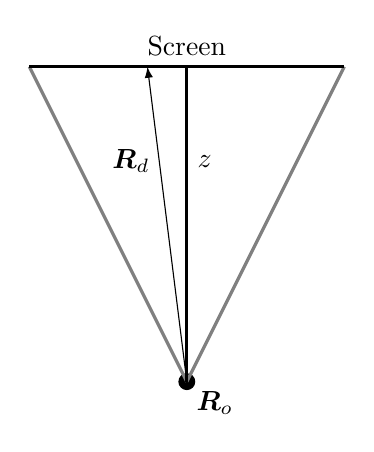
\begin{tikzpicture}
    \filldraw (0,0) circle (.1) node[anchor=north west] {$\bm R_o$};
    \draw[very thick,color=gray] (0,0) -- (-2,4);
    \draw[very thick,color=gray] (0,0) -- (2,4);
    \draw[very thick] (-2,4) -- (2,4) node[anchor=south,pos=.5]
        {Screen};
    \draw[very thick] (0,0) -- (0,4) node[anchor=west,pos=.7]
        {$z$};
    \draw[-latex] (0,0) -- (-.5,4) node[anchor=east,pos=.7] {$\bm R_d$};
\end{tikzpicture}

With $\theta$ = x angle, $\phi$ = y angle:
\begin{gather*}
    \theta = \frac{x}{w} f - \frac{f}{2}\\
    \phi = \frac{y}{h} f - \frac{f}{2}\\
    p_x = \sin(\theta)\\
    p_y = \sin(\phi)\\
    \bm R_d = [p_x,p_y,1,0]^T
\end{gather*}

\subsubsection{Shadows}

Shadows can be implemented by casting a ray from the original ray
intersection point towards each light, and determining if they contribute
to the light at that point.

Rays will often self-intersect when checking for shadows on the surface
they start off of, which is why the new $\bm R_o$ should be equal
to $\bm R_{hit} + \epsilon \bm n$, with $\bm R_{hit}$ = ray object
intersection point, $\bm n$ = object surface normal, $\epsilon$ =
some small value (ex. 0.001), depending on how large objects typically
are.

For light sources that have area, cast multiple rays to different spots
on the light source and take the fraction of the rays that hit the light.

\includegraphics{images/epsilon-vs-no-epsilon.jpeg}

\subsubsection{Reflection}

\includegraphics[scale=2]{images/reflection.png}

For reflection, the result ray $\bm R$ is expressed as
$\bm R = \bm V - 2(\bm V \cdot \bm N) \bm N$.

Amount of reflection in traditional raytracing is determined by some
constant $k_s$ which gave the final pixel color as $c_p = k_sc_m
+ (1-k_s)c_r$, with $c_p$ = final pixel color, $c_m$ = material color,
$c_r$ = color the reflected ray returns.

Fresnel discovered that reflections at a grazing angle reflected more,
and Schlick approximated $R(\theta) = R_0 + (1-R_0)(1-\cos(\theta))^5$,
with $R(\theta)$ = reflectiveness, $R_0$ = base reflectiveness.

Ideally a raytracer should cast multiple rays with slight variation in
the same general direction and take the average of their resulting colors
when reflecting to render a more realistic surface.

\subsubsection{Refraction}

\includegraphics[scale=.5]{images/refraction.png}

Snell-Descartes law states $n_i \sin(\theta_i) = n_T \sin(\theta_T)$
\[ \frac{\sin(\theta_T)}{\sin(\theta_i)} = \frac{n_i}{n_T} = n_r \]

$n_r$ is called the relative index of refraction

The vector $\bm T$ can be calculated using $\bm T = \left(n_r(\bm N \cdot
\bm I) - \sqrt{1 - n_r^2(1-(\bm N \cdot \bm I)^2)}\right) \bm N - n_r \bm I$

Similar to reflection, refraction should use the same technique of
average of multiple rays to render more realistic surfaces.

\subsubsection{Lighting}

Typically light intensity as a function of distance is expressed as
$I(x) = 1/(ax^2 + bx + c)$, with $I$ = intensity, $x$ = distance,
$a$, $b$, $c$ = positive nonzero constants.

The amount of light energy received by a surface is determined by
the angle between the light vector and surface normal: $\hat{\bm l}
\cdot \hat{\bm n}$, with $\hat{\bm l}$ = unit light vector pointing towards
the light from the surface, $\hat{\bm n}$ = unit surface normal. Combined
with falloff, $I_{in} = I_{light} \frac{\cos\theta}{r^2}$, with $\theta$
measured between light direction $\bm l$ and surface normal $\bm n$.

Directional lights are lights that are "infinitely far", such as the
sun. In that case, it's easier to model light intensity at any point
on a surface as $I_{in} = I_{light} \cos\theta$.

Spotlights typically have some angle for which there is no attenuation,
and then begin to fall off at some larger angle, combined with distance
falloff $1/r^2$.

\subsubsection{BRDF}

BRDF, or Bidirectional Reflectance Distribution Function calculates
the ratio of light coming from one direction that gets reflected
in another direction

BRDF = $f_r(\theta_i,\phi_i;\theta_0,\phi_0)$ or $f_r(\bm l,
\bm v)$, with $\bm l$ = light direction, $\bm v$ = view direction

$I_{out} = I_{in}(\bm l) f_r(\bm l, \bm v)$ where $I_{out}(\bm v)
= \frac{I_{light} \cos(\theta_i)}{r^2} f_r(\bm l,\bm v)$

$\bm l$ and $\bm v$ must be in a local coordinate system.

\includegraphics[scale=2]{images/brdf.png}

BRDF will typically be graphed with $\bm l$ constant and then
plot $I_{out}$ as a function of $\bm v$. In the plot below, the distance
from the center of the sphere represents $f_r$.

\includegraphics[scale=2]{images/brdf-plot.png}

When keeping $\bm l$ and $\bm v$ fixed, if rotation of the surface
around the normal does not change the reflection , the material is
isotropic (ex. sphere). Surfaces with strongly oriented microgeometry elements
are anisotropic (ex. brushed metal, hair, fur).

In ideal diffuse reflectance (reflectance is the same anywhere across
the object), BRDF is a constant $f_r(\bm l,\bm v) = $ const, where the
constant is typically written as $\rho/\pi$ where $\rho$ is the
albedo, a coefficient between 0 and 1 that says what fraction
of light is reflected. When $\rho$ = 0, the surface completely
absorbs the light and no light comes out, with more light being
reflected as $\rho$ increases. The constant can also be written
as $\bm k_d$, with one $\rho$ value for each RGB channel, giving
$\bm k_d = (\rho_{red}/\pi,\rho_{green}/\pi,\rho_{blue}/\pi)$.

The function for ideal diffuse reflectance is given by
$\bm L_o = \bm k_d \max(0,\bm n \cdot \bm l) L_i/r^2$,
with $\bm L_o$ = shaded color, $\bm n$ = surface normal,
$\bm l$ = light direction (towards light), $L_i$ = light intensity,
$r$ = distance from point on surface to light.

In ideal specular reflectance, the BRDF function will typically look
like a lobe:

\includegraphics[scale=.6]{images/specular-brdf.png}

The amount of light reflected is dependent on the angle between
the view direction and the reflected light direction:

\includegraphics[scale=.5]{images/brdf-specular-reflectance.png}

The function for ideal specular reflectance can then be given by
$\bm L_o = \bm k_s (\bm v \cdot \bm r)^q L_i/r^2$, with $\bm L_o$
= output color to screen, $\bm k_s$ = specular reflection coefficient,
$q$ = specular exponent, $L_i$ = light intensity, $r$ = distance
from point on surface to light.

The specular exponent's effect can be seen in the graph below, with $\alpha$
being the angle between $\bm v$ and the $\bm r$ vector (above diagram)
and the vertical axis representing the output intensity:

\includegraphics[scale=.5]{images/specular-exponent-graph.png}

\subsubsection{Phong lighting model}

Phong lighting model is made up of ambient, diffuse, and specular
light. Ambient light is the base color of objects when all lights
are off, diffuse is light intensity and angle dependent
which gives a rough surface look, specular light adds shininess.

The equation for the phong lighting model can be given by:
\[
    \bm L_o = \left(\bm k_a + \bm k_d(\bm n \cdot \bm l) + \bm k_s
    (\bm v \cdot \bm r)^q\right) \frac{L_i}{r^2}
\]

What the variables represent are listed in the previous BRDF subsection.

The chart below shows the BRDF graphs of lights at different $\phi$
angles from the vertical axis:

\includegraphics{images/phong-brdf-shapes.png}

One issue with phong is that it doesn't capture higher specular
reflection at grazing angles, which is what the Blinn-Torrance phong
variation attempts to solve.

\includegraphics[scale=.5]{images/blinn-torrance.png}

\[ \bm L_{o,s} = \bm k_s (\bm n \cdot \bm h)^q \frac{L_i}{r^2} \]

where
\[ \bm h = \frac{\bm l + \bm v}{||\bm l + \bm v||} \]

Specular BRDF lobe comparison (Blinn-Torrance vs phong):

\includegraphics[scale=.5]{images/phong-blinn-lobe-comparison.png}

The half vector lobe is preferable because it's more consistent with
what is observed in real world measurments.

\subsubsection{Normal interpolation}

Normal interpolation gives the illusion that a triangle mesh
is smoother than it actually is. For any point on a triangle
in the triangle mesh, get its barycentric coordinates and multiply
them by the vertex normals of the three triangle vertices. Remember
to renormalize normals after interpolation.
$\bm n(\alpha,\beta,\gamma) = \alpha \bm n_0 + \beta \bm n_1 + \gamma \bm n_2$

\subsubsection{Textures}

Each vertex on a triangle will contain $(u,v)$ coordinates which
indicate where it is on the texture, which can then be interpolated
with barycentric coordinates to give the texture at any point on the
triangle.

\includegraphics[scale=.5]{images/texture-map.png}

This technique of texture interpolation can also be used for normals.

\subsubsection{Skybox}

If a casted ray intersects nothing, use the skybox color instead. Cast a ray in the same
direction inside of a unit cube. The longest dimension of the ray direction determines which
side the ray will hit, and which other two dimensions are used to determine $u$ and $v$ coordinates
of the texture on that side.

For example, if the longest dimension is $x$, the sides of the skybox that can be intersected are
$-x$ and $+x$. Then $u$ and $v$ can be determined from $y$ and $z$ using $\frac{\Delta x}{x} =
\frac{\Delta y}{y} = \frac{\Delta z}{z}$, with $\Delta x = \sign(x)/2$.

\subsection{Optimization}

\subsubsection{Bounding volume: Axis-aligned bounding box}

A bounding volume encloses an object entirely, and if a ray
doesn't intersect the bounding volume it will not attempt to
check for intersections with the more complicated object.

\includegraphics[scale=2]{images/bounding-volume.png}

Box can be described as $(x_1,y_1,z_1) \rightarrow (x_2,y_2,z_2)$ where
$x_1 < x_2$, $y_1 < y_2$, $z_1 < z_2$. To check if a ray intersects
with the bounding box, check intervals of $t$ for which the ray is
within the range of the bounding box.

After the three intervals of $t$ for dimensions x, y, and z have been
determined, the starting point of intersection $t_{start}$ is the max of the mins
and the ending point of the intersection $t_{end}$ is the min of the maxes.
If $t_{start} > t_{end}$, there is no intersection.

\subsubsection{Bounding volume hierarchy (BVH)}

A bounding volume might not be enough for optimization if the object
it encloses has a large number of triangles, which a BVH solves by
splitting objects into two and calculating bounding volumes of the smaller
sections of the object. Each sub bounding volume will then create its
own two smaller bounding volumes, and eventually a binary tree will
be created of bounding volumes.

The best way to split bounding volumes is typically to sort all triangles
according to one dimension and splitting that list in half to create
two new bounding volumes.

When intersecting with bounding volumes, the first bounding volume
intersected is not necessarily the only one that needs to be intersected.
What determines that is if the ray intersects with a triangle.

Bounding volumes are allowed to intersect with each other in a BVH.

\subsubsection{Kd-trees}

Each space splits itself into two parts somewhere that neatly
divides objects into two spaces. Unlike BVH, Kd-tree partitions do not overlap.

\includegraphics{images/kd-tree.png}

Kd-tree construction
\begin{itemize}
    \item Start with scene AABB
    \item Decide which dimension to split on (longest dimension is
        typically good)
    \item Decide distance to split
    \begin{subitemize}
        \item It may be impossible to get a clean split, in which
            case any objects overlapping the boundary should be considered
            to be part of both spaces
    \end{subitemize}
    \item Stop when a minimum number of primitives is reached
    \begin{subitemize}
        \item Other criteria can be used as well
    \end{subitemize}
\end{itemize}

Kd-tree traversal
\begin{itemize}
    \item If leaf, intersect with contained primitives. If no intersection
        continue as normal.
    \item If any of the two children, intersect with those children recursively
\end{itemize}

\subsection{Advanced techniques}

\subsubsection{Global illumination}

In simple raytracing, a ray is cast towards each light from the
intersection point. In global illumination, a ray is cast towards
every direction on the hemisphere.

\includegraphics[scale=.5]{images/reflectance-equation.png}

Reflectance equation, with $L_{out}$ = outgoing light in direction
$\bm v$, $\bm x$ = intersection point,
\[ L_{out} = \int_{\Omega} L_{in}(\bm l) f_r(\bm x,\bm l,\bm v)
\cos\theta \dif \bm l \]

The full rendering equation just includes light sources in $E_{out}$,
which is 0 if not a light source:
\[ L_{out} = \int_{\Omega} L_{in}(\bm l) f_r(\bm x,\bm l,\bm v)
\cos\theta \dif \bm l + E_{out}(\bm x,\bm v) \]

Analytical solution to rendering equation is usually impossible;
however, there are many ways to solve it approximately.

Monte-Carlo raytracing: Cast a single ray per pixel, and have the ray generate
multiple new rays for every intersection in the scene. After some recursion
limit is hit, each final ray casts a ray towards each light source.

Monte-Carlo pathtracing: Cast multiple rays per pixel, and have the ray
generate only one ray for every intersection in the scene. After some
recursion limit is hit, the final ray casts a ray towards each light source.

The scene will typically be very noisy when rendered with Monte-Carlo methods,
because they randomly generate rays within a hemisphere, which can be
fixed with more samples.

\subsubsection{Irradiance caching, photon mapping}

In irradiance caching, because indirect illumination is smooth, the indirect light of multiple points
in the scene can be sampled and then indrect light in between the points can be
interpolated.

\includegraphics[scale=.5]{images/irradiance-cache.png}

Yellow points indicate points which were sampled for irradiance caching,
notably around sharp features because that's where indirect illumination
is not smooth.

Photon mapping is similar to irradiance caching, but instead of having
the camera cast rays to sample points, the light casts random rays
and the points from that are used.

\includegraphics[scale=.5]{images/photon-mapping.png}

When accessing the data of irradiance caching or photon mapping, a hierarchical
structure like a kd-tree is required because of the large number of data
points to look through.

\subsubsection{Monte-Carlo integration}

\includegraphics[scale=.4]{images/monte-carlo-integration.png}

Take random samples and find the average
\[ \int_S f(x) \dif x \approx \frac{V(S)}{N} \sum_{i=1}^N f(x_i) \]

where $S$ is the integration domain, $V(S)$ is the volume of $S$, $x_i$
are random x values and $N$ is the number of random samples.

The average error is proportional to $1/\sqrt{N}$, which means 4x the number
of samples is required to halve the error.

One disadvantage of Monte-Carlo integration is that it's very noisy, which
importance sampling partially fixes. When sampling a BRDF function, it's better
to sample areas that will contribute to the integral more, because they will
make the largest difference depending on whether they're sampled or not.

\includegraphics[scale=.4]{images/importance-sampling.png}

Importance sampling can be represented by
\[ \int_S f(x) \dif x \approx \frac{V(S)}{N} \sum_{i=1}^N \frac{f(x_i)}{p(x_i)} \]

where $p$ is some probability distribution.

\section{Rasterization}

In rasterization, geometry (often triangles) are projected onto the screen using their vertices,
and then interpolating the pixels in between the vertices.

\subsection{Z-buffer}

When there is a pixel that is a part of multiple objects, determining which one is nearest requires
a z-buffer, which contains depth information of each pixel on the screen.

\subsubsection{Interpolating z values}

Scanline rendering iterates over all y values (screen space) from the highest vertex to
the lowest vertex, taking two points on opposite sides on the edges of the triangle for
each y value.

\end{document}
